% =========================================================================
% ICDEES 2026 Conference Paper Manuscript (IEEE Format)
% Venue: International Conference on Digital Economy and Emerging Societies (ICDEES 2026)
% IEEE Proceedings / IEEE Xplore Indexing
% Formatting: IEEEtran Conference (Double-Blind Review Ready)
% Structure: IMRaD (Introduction, Method, Result, Discussion, Conclusion)
% Target Length: Strictly 6 Pages Maximum (No Page 7 Spillover)
% =========================================================================

\documentclass[conference]{IEEEtran}
\IEEEoverridecommandlockouts

% -------------------------------------------------------------------------
% Core Packages & Typographical Optimization
% -------------------------------------------------------------------------
\usepackage{cite}
\usepackage{amsmath,amssymb,amsfonts}
\usepackage{algorithmic}
\usepackage{algorithm}
\usepackage{graphicx}
\usepackage{textcomp}
\usepackage{xcolor}
\usepackage{booktabs}
\usepackage{array}
\usepackage{adjustbox}
\usepackage{url}
\usepackage{microtype}
\usepackage[letterpaper, top=0.80in, bottom=1.04in, left=0.68in, right=0.68in, columnsep=0.25in]{geometry}
\raggedbottom

% -------------------------------------------------------------------------
% Float Spacing Adjustments (Guarantees Strict 6-Page Fit)
% -------------------------------------------------------------------------
\setlength{\textfloatsep}{3.5pt plus 1pt minus 1pt}
\setlength{\floatsep}{2.5pt plus 1pt minus 1pt}
\setlength{\intextsep}{2.5pt plus 1pt minus 1pt}
\setlength{\abovecaptionskip}{2pt plus 0.5pt minus 0.5pt}
\setlength{\belowcaptionskip}{1.5pt plus 0.5pt minus 0.5pt}

% -------------------------------------------------------------------------
% TikZ Graphics
% -------------------------------------------------------------------------
\usepackage{tikz}
\usetikzlibrary{shapes.geometric, arrows.meta, positioning, calc, fit}

% -------------------------------------------------------------------------
% Graphics Search Paths
% -------------------------------------------------------------------------
\graphicspath{{charts_ieee/}{./charts_ieee/}{charts/v03/}{./charts/v03/}{src/v3-run/}{../../src/v3-run/}}

% -------------------------------------------------------------------------
% Keyword Header Renaming (Replacing Index Terms with Keywords)
% -------------------------------------------------------------------------
\renewcommand\IEEEkeywordsname{Keywords}

\begin{document}

% -------------------------------------------------------------------------
% TITLE & AUTHOR BLOCK (IEEE Template 2x2: Author 4 aligned with Author 2)
% -------------------------------------------------------------------------
\title{Unsupervised Dual-Path Consensus Machine Learning and Operational Policy Framework for Village Fund Expenditure Anomaly Detection}

\author{
\begin{tabular}{c@{\hspace{1.5cm}}c}
\makebox[6.8cm][c]{%
\begin{tabular}[t]{c}
\textbf{Farrell Yodihartomo} \\
\textit{School of Information Systems} \\
\textit{Bina Nusantara University}\\
Jakarta, Indonesia 11480 \\
farrell.yodihartomo@binus.edu
\end{tabular}%
}
&
\makebox[6.8cm][c]{%
\begin{tabular}[t]{c}
\textbf{Pandu Wicaksono} \\
\textit{School of Computer Science} \\
\textit{Bina Nusantara University}\\
Jakarta, Indonesia 11480 \\
pandu.wicaksono@binus.ac.id
\end{tabular}%
}
\end{tabular}
\\[0.8em]
\begin{tabular}{c@{\hspace{1.5cm}}c}
\makebox[6.8cm][c]{%
\begin{tabular}[t]{c}
\textbf{Humam Faiq} \\
\textit{Directorate of Investigation} \\
\textit{Corruption Eradication Commission (KPK)}\\
Jakarta, Indonesia \\
humam.faiq@kpk.go.id
\end{tabular}%
}
&
\makebox[6.8cm][c]{%
\begin{tabular}[t]{c}
\textbf{Charlie Yen} \\
\textit{Business Information Technology} \\
\textit{Bina Nusantara University}\\
Jakarta, Indonesia 11480 \\
charlie.yen@binus.ac.id
\end{tabular}%
}
\end{tabular}
}

\maketitle

% -------------------------------------------------------------------------
% ABSTRACT
% -------------------------------------------------------------------------
\begin{abstract}
The government of Indonesia allocates around Rp 71 trillion per year to 75,259 rural locations through the program of  \textit{Dana Desa} (Village Fund). The anti-corruption monitoring is rather reactive in nature with the trials conducted at courts 2 to 5 years after the disbursed money. Supervised ML cannot help in solving this problem due to zero ground-truth labels for the fraud at disbursed amounts in the ledgers. In this paper, using the principles of DSR methodology along with agency theory and fraud diamond, we propose and test an unsupervised Dual-Path Consensus strategy (Protocol 2) through the use of Isolation Forest (IF), Local Outlier Factor (LOF), and an 8-layer Reconstruction Dense Autoencoder (RDA) with an Operational Policy Mapping Layer in 96,778 transactions (1,363 villages, 2023–2025) in Jambi province. Compared with the protocol 1 (majority voting), our protocol 2 differentiates the local density outliers from the consensus-based multi-model approach ($\text{IF} \cap \text{RDA}$). Anomaly recall increases from 3,107 (3.12\%) to 7,153 anomalies in consensus (7.39\%), identifying the realization risk of Rp 642.85 billion (14.89\%) and budget ceiling risk of Rp 6.08 trillion (7.46\%). The operational policy mapping reflects the increase of Ghost Activities (58.1\% / 4,155) and Procurement Irregularities (32.8\% / 2,343). Longitudinal monitoring identifies 702 persistent Tier-1 villages (51.5\%) over three years. On a synthetic historical antecedent fraud benchmark ($N=10,000$, 5.0\% fraud), \textbf{Protocol 2} exhibits better performance in terms of detection recovery  (\textbf{Precision = 0.846, Recall = 0.846, F1 = 0.846, AUC-ROC = 0.912} vs. \textbf{Protocol 1} F1 = 0.568). compared to Protocol 1 F1 = 0.568. Using the DeLone and McLean IS Success Model as its basis, the approach is able to narrow down the search space for the inspectorate audit by 92.6\%, while turning neural reconstruction loss into actionable Explainable AI (XAI) field checklists.
\end{abstract}

\begin{IEEEkeywords}
Unsupervised Anomaly Detection, Dual-Path Consensus, Design Science Research, Reconstruction Autoencoder, Explainable AI, Village Fund Governance.
\end{IEEEkeywords}

% -------------------------------------------------------------------------
% SECTION I: INTRODUCTION
% -------------------------------------------------------------------------
\section{Introduction}

There is an annual allocation of around Rp 71 trillion from the Indonesian government to 75,259 village regions based on Law No. 6/2014 concerning villages ~\cite{ref1}. Yet, the extent and speed of such allocations have surpassed the capacity of local surveillance. ICW has noted 591 verdicts of corruption related to village funds as of 2024, amounting to losses of Rp 598.13 billion for the state ~\cite{ref2}. From 2015 to 2022, the Corruption Eradication Commission (ACLC KPK) has recorded 851 corruption cases, which involved 973 village apparatus members, as well as Rp 468.9 trillion worth of allocated money ~\cite{ref3}.

Moreover, national bodies started to implement preventive programs such as: KPK Trisula (Education, Prevention, Enforcement) ~\cite{ref36}; Desa Antikorupsi ~\cite{ref37}; BPKP-KPK Siswaskeudes audit instrument ~\cite{ref38}; Stranas PK 2025-2026 digital supervision ~\cite{ref39}; Monitoring Center for Prevention (MCP) ~\cite{ref40}; and jaga.id portal ~\cite{ref26}. These systems mostly work in municipal level or based on voluntary citizen whistleblowing and cannot filter unstructured, activity-level Siskeudes disbursement transactions prior to disbursement transaction clearance.

Previous studies related to rural financial oversight were concentrated either on processes ~\cite{ref4,ref5} or traditional fraud triangle ~\cite{ref6}. In the realm of public sector ML auditing, scientists prefer supervised machine learning approaches ~\cite{ref13,ref14}, but transactional data are not labeled in terms of frauds ~\cite{ref16,ref23}, which prevents supervised learning. Therefore, we apply Design Science Research (DSR) ~\cite{ref5,ref10} and design, implement and compare two types of unsupervised ML models – Dual-Path Consensus (Protocol 2) and majority voting-based ensemble (Protocol 1) for 96,778 activity-level records for 1,363 Jambi villages (2023–2025).

The province of Jambi illustrates this disparity clearly. Only 11 citizens’ grievances from the province appear at the jaga.id portal maintained by the KPK out of the total number of 761 citizen complaints (1.4\%) reported in the country~\cite{ref26}. According to panel GMM threshold model (Alfada)~\cite{ref27}, high dependency on transfer payments and inadequate citizen monitoring may cause high corruption risks~\cite{ref27}. The inspectorate office at the district level (APIP) has between 5 and 15 auditors for each district~\cite{ref12}, which renders manual audit difficult according to Government Regulation No. 60/2008~\cite{ref33}. The recent cases of legal proceedings prove discrepancies in account books: Muara Hemat (Kerinci; Rp 644 million loss; 5-year prosecution delay)~\cite{ref28,ref30}, Jambi Tulo (Muaro Jambi; Rp 300 million fictitious projects) ~\cite{ref29}; and Pangkal Duri (Tanjung Jabung Timur; Rp 415 million loss)~\cite{ref31}.

Specifically, this study provides three key contributions:
\begin{enumerate}
    \item \textbf{Methodological}: Dual-Path Consensus protocol integrating LOF and multimodel global convergence ($\text{IF} \cap \text{RDA}$), and the Policy Mapping Layer to address majority voting's mutual cancellation issues (Protocol 1).
    \item \textbf{Theoretical}: Integration of Agency Theory, Fraud Diamond, and principal-agent information asymmetry in Siskeudes administrative features.
    \item \textbf{Practical}: A screening system that can reduce the APIP audit search space by 92.6\%, locate 702 villages with a persistent Tier-1 status, and convert autoencoder losses to XAI inspection checklists.
\end{enumerate}

Finally, this study addresses three Research Questions (RQs):
\begin{itemize}
    \item \textbf{RQ1}1: What is the most effective engineered feature from Siskeudes that signals spending anomalies?
    \item \textbf{RQ2}: What is the best ensemble architecture for anomalous discrimination on longitudinal village fund data?
    \item \textbf{RQ3}: How do identified anomalies relate to corruption typologies and what is the XAI loss decomposition guideline for APIP field inspection?
\end{itemize}


% -------------------------------------------------------------------------
% SECTION II: METHODOLOGY & ARTIFACT ARCHITECTURE (IMRaD - Method)
% -------------------------------------------------------------------------
\section{Methodology and Artifacts Architecture}

\subsection{Theoretical Foundation and Conceptual Model}

The theoretical concepts behind the proposed artefact are drawn from the Fraud Diamond, agency theory, and the IS success model. The principal-agent arrangement sees the Villager Head (Kepala Desa), as an agent who has information not available to the principal (APIP inspection, BPKP, KPK):
\begin{equation}
\begin{aligned}
\mathrm{InfoAsymmetry} = {} & \mathcal{I}_{\mathrm{Agent}}(\mathrm{Realization}, \mathrm{TrueCost}) \\
& - \mathcal{I}_{\mathrm{Principal}}(\mathrm{SiskeudesReport})
\end{aligned}
\end{equation}
For the case of implementation of Siskeudes, \textbf{Capability} belongs to the Village Head and the Financial Officer (Kaur Keuangan) who have responsibility for management of digital certificates and specimen signatures for bank authorization. \textbf{Opportunity} exists in the procurement process because 98.8\% of all village fund operations in Jambi Province are managed through Swakelola procurement without competition \cite{ref9}.

The process of Siskeudes implementation includes the exercise of \textbf{Capability} by the Village Head and the Financial Officer (Kaur Keuangan). They are responsible for digital certificates and specimen signatures used for bank authorization. \textbf{Opportunity} exists in the procurement process because 98.8\% of all village fund operations in Jambi Province are managed through Swakelola procurement without competition \cite{ref9}.

\begin{figure}[htbp]
\centering
\resizebox{\columnwidth}{!}{%
\begin{tikzpicture}[
    box/.style={draw=black!70, rectangle, rounded corners=3pt, align=center, minimum height=0.85cm, minimum width=2.0cm, fill=blue!5, font=\sffamily\scriptsize, line width=0.7pt},
    arrow/.style={-Stealth, thick, color=black!80, line width=0.9pt}
]
    \node[box, fill=red!10] (problem) {\textbf{Problem Domain}\\Rural Governance Deficit\\Siskeudes Signal Archive};
    \node[box, fill=amber!10, right=0.4cm of problem] (theory) {\textbf{Theory Foundation}\\Agency Asymmetry~\cite{ref25}\\Fraud Diamond~\cite{ref17b}};
    \node[box, fill=blue!10, right=0.4cm of theory] (artifact) {\textbf{DSR Artifact}\\Protocol 1: Majority\\Protocol 2: Dual-Path};
    \node[box, fill=green!10, right=0.4cm of artifact] (impact) {\textbf{IS Success Impact}\\92.6\% Search Reduction\\APIP Checklist~\cite{ref10}};

    \draw[arrow] (problem) -- (theory);
    \draw[arrow] (theory) -- (artifact);
    \draw[arrow] (artifact) -- (impact);
\end{tikzpicture}%
}

\caption{Integrated Conceptual Framework linking Agency Theory, Fraud Diamond, DSR Comparative Artifacts, and DeLone \& McLean IS Success Impact.}
\label{fig:conceptual_framework}
\end{figure}

\subsection{Data Hygiene \& Regional Baseline Centering}

Dataset in its raw form (99,692 observations) is gathered by KPK jaga.id ~\cite{ref26} and consists of expenditure absorption (\textit{Penyerapan}) and budget ceiling (\textit{Pagu}) ledgers for fiscal years 2023-2025. Data cleansing procedure excludes zero volume and faulty codes, producing N = 96,778 valid observations from 1,363 villages.

In order to control for baseline price inflation caused by harsh mountainous terrain and expensive logistics costs (for example, Kerinci highlands compared to Muaro Jambi lowlands), z-scores per region are calculated year-by-year 
$(c, k, t) = (\text{Kode\_Output}, \text{Kabupaten\_Kota}, \text{Tahun})$:
\begin{equation}
z_{i,c,k,t} = \frac{x_{i,c,k,t} - \mu_{c,k,t}}{\sigma_{c,k,t} + \epsilon}
\end{equation}
RobustScaler (median-based standardization with IQR scale) is applied to continuous variables to reduce the effect of outliers on price. The feature matrix used contains 27 variables, which is shown in Table \ref{tab:feature_matrix}.

\begin{table}[htbp]
\centering
\caption{27-Variable Feature Engineering Matrix and Targeted Modus Operandi}
\label{tab:feature_matrix}
\setlength{\tabcolsep}{2.5pt}
\resizebox{\columnwidth}{!}{%
\begin{tabular}{lll}
\toprule
\textbf{Feature Construct} & \textbf{Mathematical Definition} & \textbf{Targeted Modus Operandi} \\
\midrule
\texttt{cost\_per\_unit} & $\text{Realization\_Total}_i / \text{Volume}_i$ (RobustScaler) & Unit price mark-up / inflation (T1) \\
\texttt{absorption\_ratio} & $\text{Realization\_Total}_i / \text{Pagu\_Village}_{v,t}$ & Ghost activity / zero progress (T2) \\
\texttt{avg\_completion} & $\frac{1}{3}(\text{Pct\_T1}_i + \text{Pct\_T2}_i + \text{Pct\_T3}_i)$ & Progress reporting manipulation \\
\texttt{swakelola\_high\_val} & $\mathbf{1}\left(\text{Swakelola}_i \land \text{Realization}_i > Q_{0.75}\right)$ & Uncompetitive procurement (T5) \\
\texttt{cost\_dev\_by\_cat} & $z_{i,c,k,t} = (x_{i,c,k,t} - \mu_{c,k,t}) / \sigma_{c,k,t}$ in $(c,k,t)$ & Regional price outlier (T7) \\
\texttt{n\_stages\_active} & $\sum_{m=1}^{3} \mathbf{1}\left(\text{Real\_T}m_i > 0\right)$ & Tranche draw concentration (T4) \\
\texttt{activity\_category} & One-Hot Encoded \texttt{Kode\_Output} (21 cats) & Cross-category dumping (T7) \\
\bottomrule
\end{tabular}%
}
\end{table}

\subsection{Multi-Paradigm Unsupervised Detection Engines}

The framework implements three orthogonal detection paradigms:

\subsubsection{1. Isolation Forest (Global Sparsity Engine)}

Isolation Forest divides the feature space through recursive splits \cite{ref18}. The number of splittings required to isolate each instance x in T = 200 trees is called the path length h(x), while the anomaly score for each sample is $s(x, n) = 2^{-\mathbb{E}(h(x))/c(n)}$ where contamination c = 0.10.
\begin{equation}
y_{i, \mathrm{IF}} = \mathbf{1}\left(s(x_i, n) \ge \mathrm{Quantile}_{0.90}(s)\right)
\end{equation}

\subsubsection{2. Local Outlier Factor (Density Ratio Engine)}

LOF calculates the ratio of the local reachability density ($\text{lrd}_k$) of instance $p$ to that of its 20 nearest neighbours $k$~\cite{ref24}:
\begin{equation}
\mathrm{LOF}_k(p) = \frac{1}{|N_k(p)|} \sum_{o \in N_k(p)} \frac{\mathrm{lrd}_k(o)}{\mathrm{lrd}_k(p)}
\end{equation}
\begin{equation}
y_{i, \mathrm{LOF}} = \mathbf{1}\left(\mathrm{LOF}_k(x_i) \ge \mathrm{Quantile}_{0.95}(\mathrm{LOF})\right)
\end{equation}

\subsubsection{3. Reconstruction Dense Autoencoder (RDA \& Neural Loss)}
In RDA, the number of layers in the symmetric bottleneck neural network model is eight, as specified by the structure:  \texttt{[27 -> 64 -> 32 -> 16 -> 8 -> 16 -> 32 -> 64 -> 27]} with MSE loss function and L2 regularization with ($\lambda = 1\times 10^{-3}$) as stated in reference ~\cite{ref32}. The overall error for instance $i$ is represented as $E_i$, while $e_{i,f}$ represents the error fraction for feature f.
\begin{equation}
E_i = \sum_{f=1}^{d} (x_{i,f} - \hat{x}_{i,f})^2, \quad e_{i,f} = \frac{(x_{i,f} - \hat{x}_{i,f})^2}{E_i}
\end{equation}
\begin{equation}
y_{i, \mathrm{RDA}} = \mathbf{1}\left(E_i \ge \mathrm{Quantile}_{0.95}(E)\right)
\end{equation}

\subsection{Dual-Path Consensus Ensemble Gate}

Protocol 1 (baseline) used majority voting ($\sum \text{Flag}_m \ge 2$) to generate considerable mutual cancellation, by ignoring the localized density isolates, which were not consistent with the global tree partitions. The Dual-Path Consensus Ensemble Gate of Protocol 2, however, disassociates local density determination from multi-model global convergence as follows:

\begin{equation}
y_{i, \mathrm{consensus}} = y_{i, \mathrm{LOF}} \lor \left(y_{i, \mathrm{IF}} \land y_{i, \mathrm{RDA}}\right)
\end{equation}

The gate determines 7,153 consensus anomalies, representing 7.39\% of total observations, of which 3,940 belong to local density isolates and 2,314 to global multi-model convergence.

\begin{algorithm}[htbp]
\caption{End-to-End Dual-Path Anomaly Detection \& XAI Pipeline}
\label{alg:end_to_end}
\begin{algorithmic}[1]
\REQUIRE Raw Records $\mathcal{D}$, Contamination $c=0.10$, LOF $k=20$, RDA bottleneck $h=8$, Quantile $q=0.95$.
\ENSURE Consensus Vector $\mathbf{y}_{\text{cons}}$, Typologies $\{\mathcal{T}_i\}$, XAI Checklists $\{\mathcal{C}_i\}$.
\STATE \textbf{Data Hygiene \& Centering:} Purge zero-volume records; compute within-stratum z-score $z_{i, \text{cat}} = (x_i - \mu_{c,k,t})/(\sigma_{c,k,t}+\epsilon)$; scale via RobustScaler $\to \mathbf{X} \in \mathbb{R}^{N \times d}$.
\STATE \textbf{Multi-Paradigm Inference:} Fit IF ($y_{i,\text{IF}}$), LOF ($y_{i,\text{LOF}}$), and RDA ($y_{i,\text{RDA}}$).
\STATE \textbf{Dual-Path Gating:} $y_{i, \text{cons}} \leftarrow y_{i, \text{LOF}} \lor (y_{i, \text{IF}} \land y_{i, \text{RDA}})$.
\FOR{each flagged instance $x_i$ where $y_{i, \text{cons}} = 1$}
    \STATE Map $\mathcal{T}_i$ via rules: $T_1$ (Mark-Up), $T_2$ (Ghost), $T_5$ (Procurement), $T_7$ (Dumping), or Unclassified Risk.
    \STATE Decompose error $e_{i,f} \leftarrow (x_{i,f} - \hat{x}_{i,f})^2 / E_i$; rank features descending to build audit checklist $\mathcal{C}_i$.
\ENDFOR
\RETURN $\mathbf{y}_{\text{cons}}$, $\{\mathcal{T}_i\}$, $\{\mathcal{C}_i\}$.
\end{algorithmic}
\end{algorithm}

% -------------------------------------------------------------------------
% SECTION III: RESULTS (IMRaD - Result)
% -------------------------------------------------------------------------
\section{Results \& Empirical Analysis}

\subsection{Anomaly Flag Counts per Method \& Consistency of Rate}

Table~\ref{tab:flag_counts} provides the comparison of anomaly detection flag counts for Protocol 1 and Protocol 2. Fig.~\ref{fig:consistency} shows the yearly consistency in rate of anomaly flags in the active years 2023 through 2025.

\begin{table}[htbp]
\centering
\caption{Per-Method Anomaly Flag Counts and Overall Rates (\textbf{Protocol 1} vs \textbf{Protocol 2})}
\label{tab:flag_counts}
\setlength{\tabcolsep}{2.5pt}
\resizebox{\columnwidth}{!}{%
\begin{tabular}{lcccc}
\toprule
\textbf{Detection Paradigm} & \textbf{P1 Count} & \textbf{P1 \%} & \textbf{P2 Count} & \textbf{P2 \%} \\
\midrule
Isolation Forest (IF) & 7,974 & 8.00\% & 9,678 & 10.00\% \\
Local Outlier Factor (LOF) & 4,985 & 5.00\% & 4,839 & 5.00\% \\
Reconstruction DA (RDA) & 4,985 & 5.00\% & 4,840 & 5.00\% \\
\textbf{Consensus Flag (Ensemble)} & \textbf{3,107} & \textbf{3.12\%} & \textbf{7,153} & \textbf{7.39\%} \\
\bottomrule
\end{tabular}%
}
\end{table}

\begin{figure}[htbp]
\centering
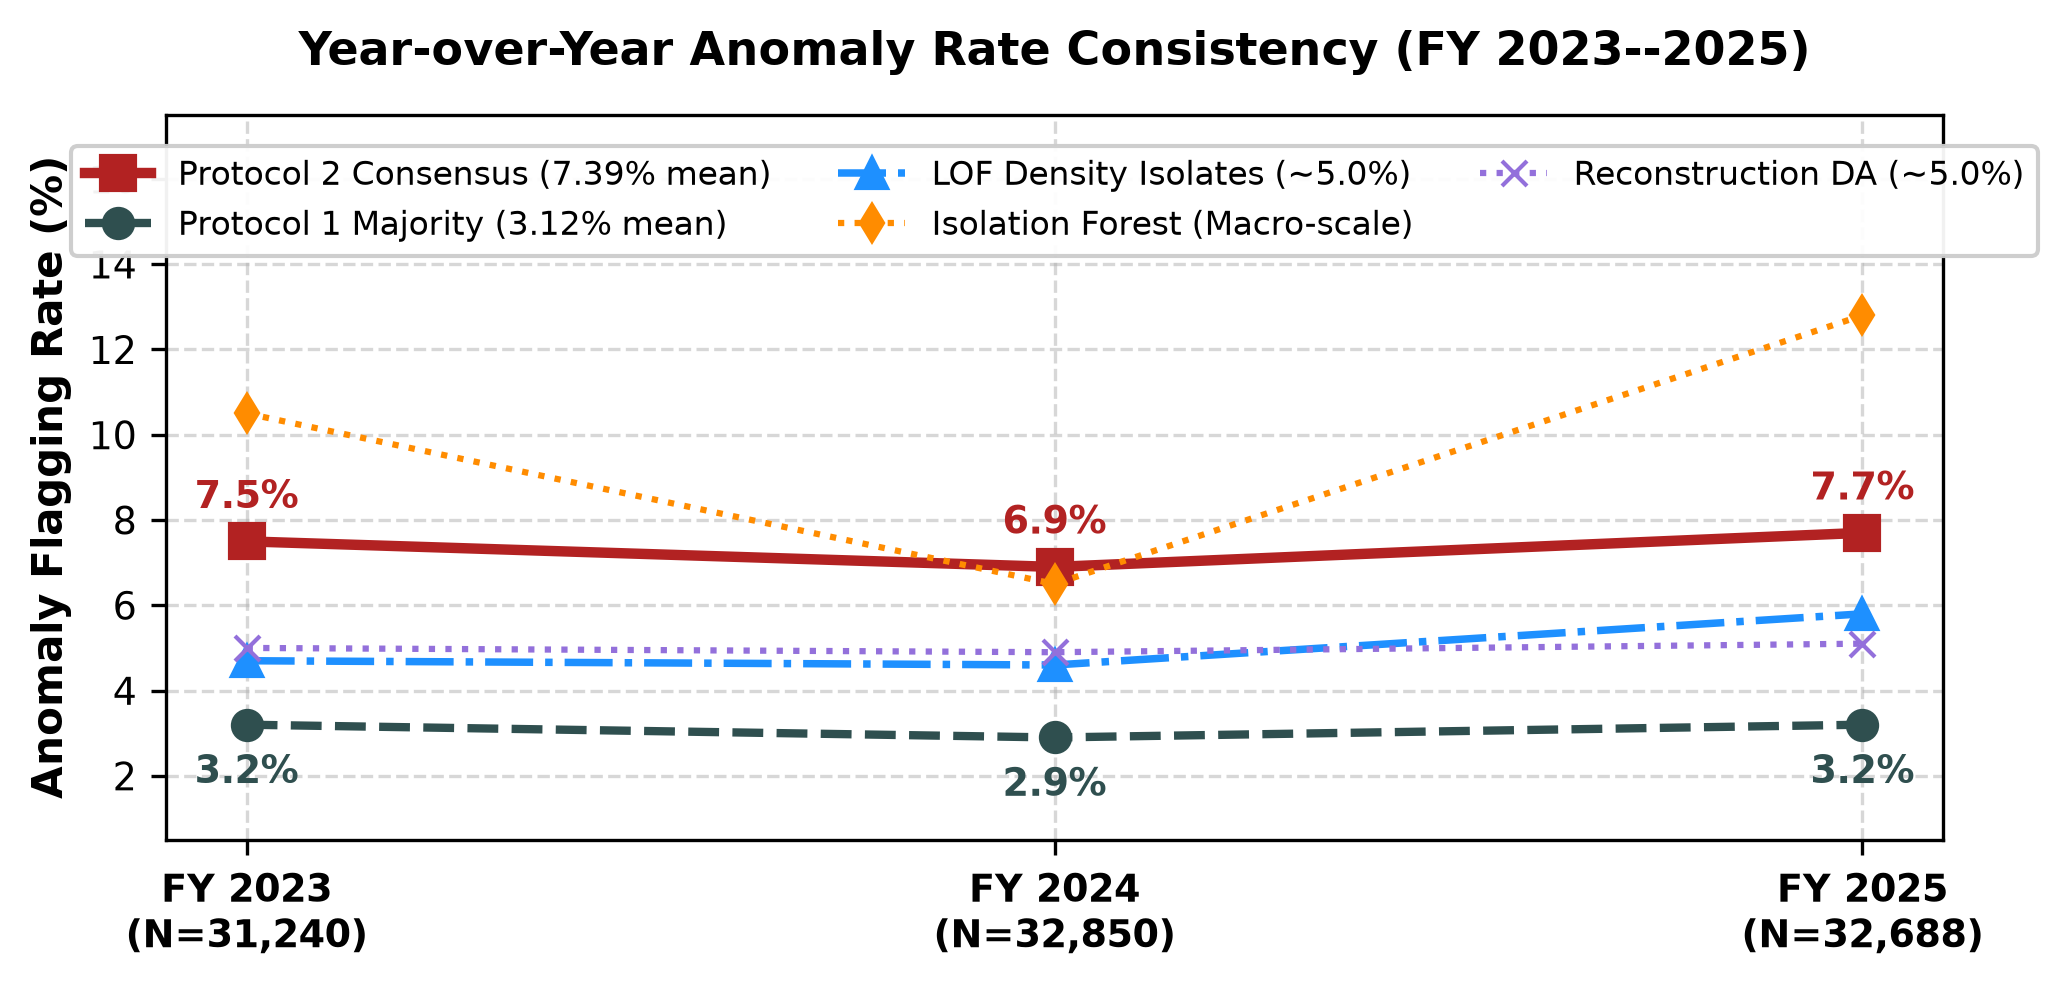
\includegraphics[width=\columnwidth]{charts_ieee/ieee_rate_consistency.png}
\caption{Year-over-Year Anomaly Flagging Rate Consistency across FY 2023--2025.}
\label{fig:consistency}
\end{figure}

From Fig.~\ref{fig:consistency}, LOF provides a consistent flagging rate each year (4.7\% in 2023 $\to$ 4.6\% in 2024 $\to$ 5.8\% in 2025) by adjusting to the annual budget changes smoothly.

\subsection{Score Distribution Shape \& Subspace Orthogonality}

Fig.~\ref{fig:distributions} and Table~\ref{tab:bimodality_overlap} evaluate score distributions annotated with Sarle Bimodality Coefficients (BC) and pairwise Cohen's $\kappa$.

\begin{figure}[htbp]
\centering
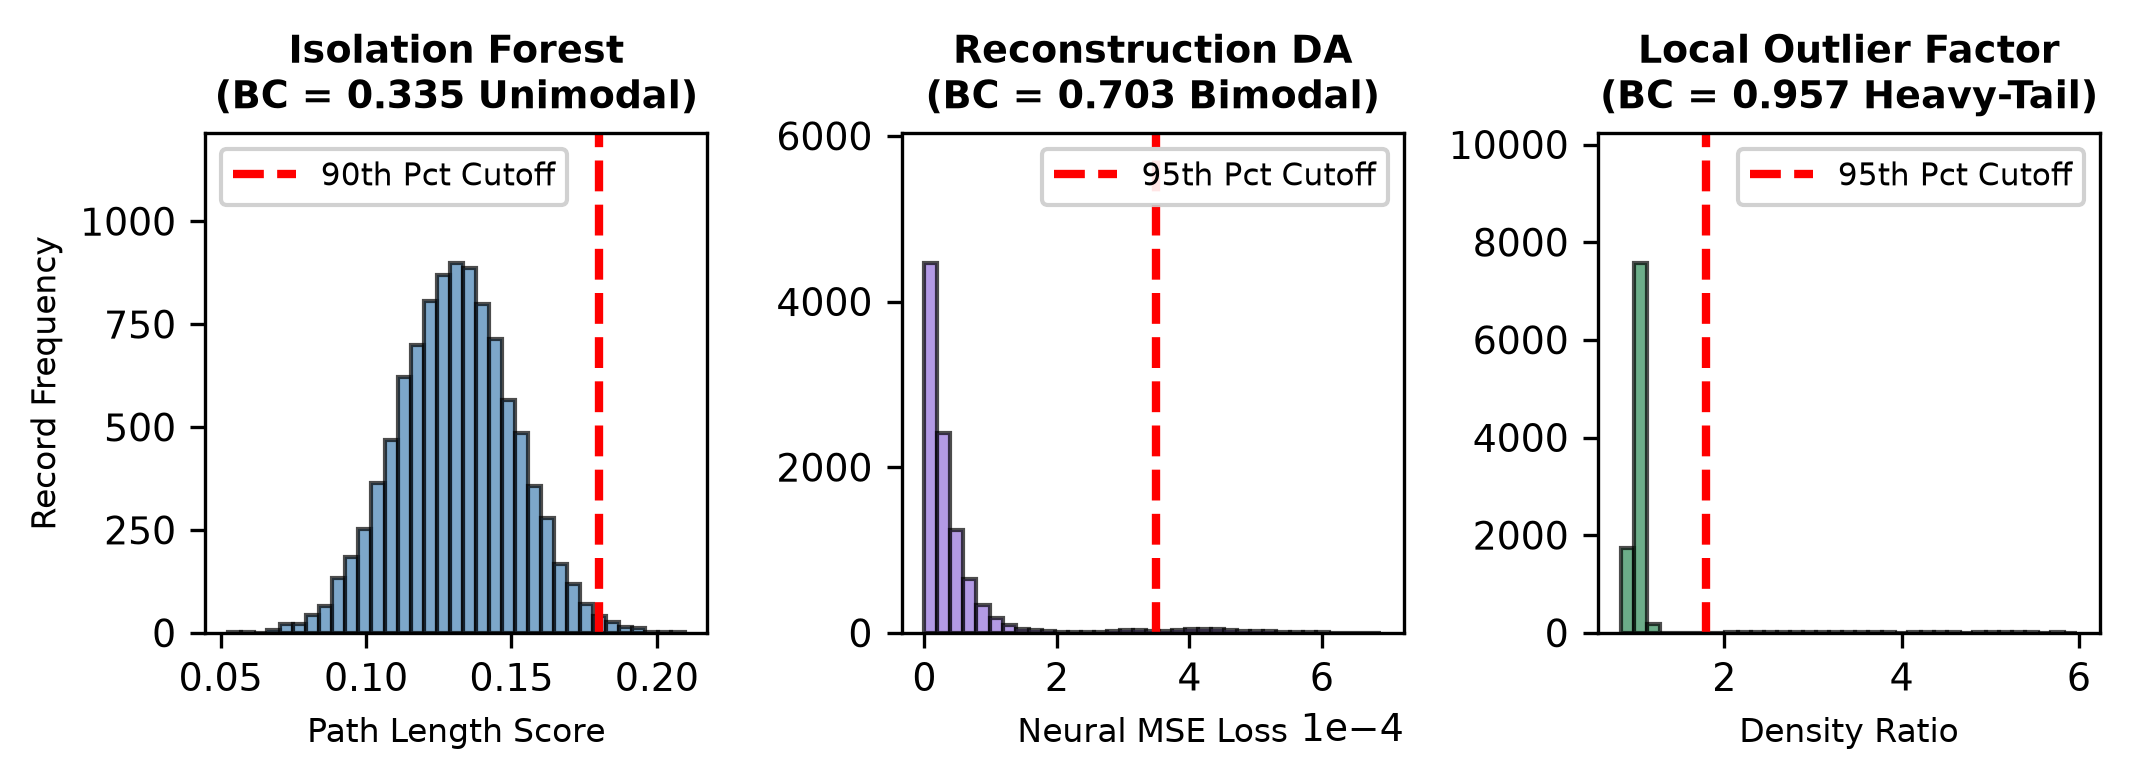
\includegraphics[width=\columnwidth]{charts_ieee/ieee_score_distributions.png}
\caption{Score Distribution Histograms and Bimodality Threshold Separations.}
\label{fig:distributions}
\end{figure}

\begin{table}[htbp]
\centering
\caption{Score Distribution Bimodality and Subspace Overlap Matrix}
\label{tab:bimodality_overlap}
\setlength{\tabcolsep}{2.5pt}
\resizebox{\columnwidth}{!}{%
\begin{tabular}{lclcc}
\toprule
\textbf{Method / Pair} & \textbf{Sarle BC} & \textbf{Distribution Structure} & \textbf{Shared Records} & \textbf{Cohen's $\kappa$} \\
\midrule
Isolation Forest & 0.335 & Unimodal continuous spectrum & --- & --- \\
Reconstruction DA & \textbf{0.703} & Moderate bimodal (clear tail) & --- & --- \\
Local Outlier Factor & \textbf{0.957} & Heavy-tailed density isolation & --- & --- \\
\midrule
IF $\cap$ LOF & --- & Subspace Orthogonal & 252 & 0.041 (Slight) \\
IF $\cap$ RDA & --- & Global Convergence & 2,314 & \textbf{0.482 (Mod.)} \\
LOF $\cap$ RDA & --- & Subspace Orthogonal & 422 & 0.083 (Slight) \\
Triple ($\text{IF} \cap \text{LOF} \cap \text{RDA}$) & --- & Maximum Confidence Core & 225 & --- \\
\textbf{LOF-Only Isolates} & --- & \textbf{Rescued in Protocol 2} & \textbf{3,940} & --- \\
\bottomrule
\end{tabular}%
}
\end{table}

In the case of LOF, a Sarle Bimodality Coefficient (BC) of 0.957 is achieved and hence able to clearly differentiate between normal clusters and density outliers up to $5.40 \times 10^9$. From table ~\ref{tab:bimodality_overlap}, it shows that the detectors are functioning in orthogonal subspaces where 3,940 data points are detected by LOF only.

% ---------------- FROM HERE

\subsection{Corruption Typology Mapping \& Shift Dynamics}

Consensus flags were mapped into domain-grounded corruption typologies via Algorithm~\ref{alg:end_to_end}. Fig.~\ref{fig:typology} and Table~\ref{tab:typology_shift} detail the dramatic typology shift from Protocol 1 to Protocol 2.

\begin{figure}[htbp]
\centering
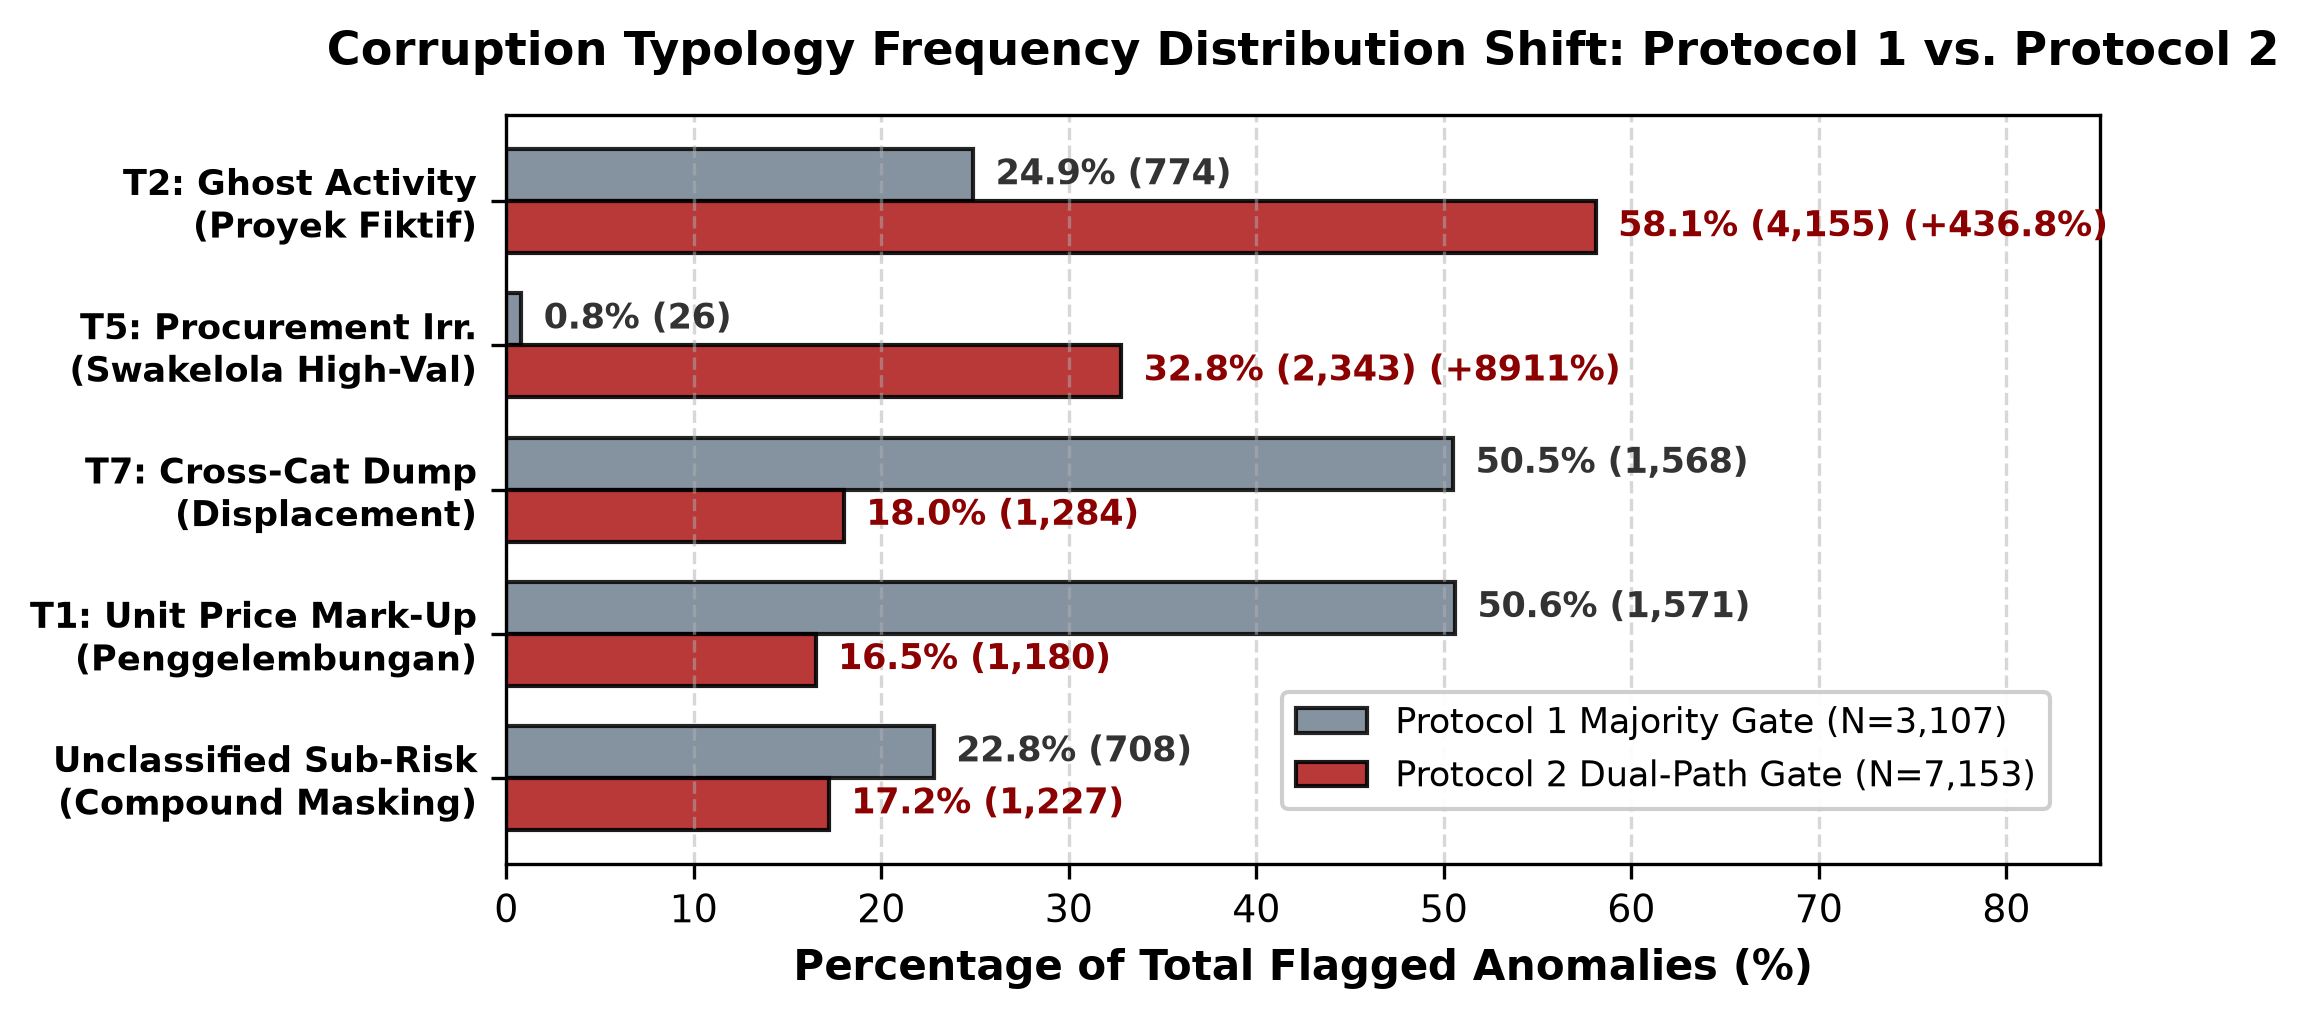
\includegraphics[width=\columnwidth]{charts_ieee/ieee_typology_comparison.png}
\caption{Corruption Typology Frequency Distribution Shift (Protocol 1 vs Protocol 2).}
\label{fig:typology}
\end{figure}

\begin{table}[htbp]
\centering
\caption{Comparative Typology Frequency Shift (\textbf{Protocol 1} vs \textbf{Protocol 2})}
\label{tab:typology_shift}
\setlength{\tabcolsep}{2.5pt}
\resizebox{\columnwidth}{!}{%
\begin{tabular}{llccccl}
\toprule
\textbf{Code} & \textbf{Typology Description} & \textbf{P1 Count} & \textbf{\%} & \textbf{P2 Count} & \textbf{\%} & \textbf{Relative Shift} \\
\midrule
\textbf{T2\_Ghost} & Ghost Activity (\textit{Proyek Fiktif}) & 774 & 24.9\% & \textbf{4,155} & \textbf{58.1\%} & \textbf{+436.8\% (Primary)} \\
\textbf{T5\_Procure} & Procurement Irr. (\textit{Swakelola}) & 26 & 0.8\% & \textbf{2,343} & \textbf{32.8\%} & \textbf{+8911.5\% (Major)} \\
\textbf{T7\_Dump} & Cross-Category Dumping & 1,568 & 50.5\% & \textbf{1,284} & \textbf{18.0\%} & $-$18.1\% (Refined) \\
\textbf{T1\_Markup} & Unit Price Mark-Up (\textit{Mark-up}) & 1,571 & 50.6\% & \textbf{1,180} & \textbf{16.5\%} & $-$24.9\% (Refined) \\
\textbf{T4\_Lock} & Disbursement Stage Lock & 0 & 0.0\% & \textbf{28} & \textbf{0.4\%} & Newly captured \\
\textbf{Unclassified} & Sub-threshold Masking & 708 & 22.8\% & \textbf{1,227} & \textbf{17.2\%} & Proportional drop \\
\bottomrule
\end{tabular}%
}
\end{table}

\textbf{Protocol 2} creates two dominant corruption types: \textbf{T2: Ghost Activities (58.1\% / 4,155 records)}  and \textbf{T5: Procurement Irregularities (32.8\% / 2,343 records)}.

\subsection{XAI Reconstruction Error Drivers \& Spatial Clustering}

Figure \ref{fig:rda_error} shows RDA error per feature breakdown with \texttt{cost\_dev\_by\_cat} (which is the key factor in 2,065 observations or 42.7\%) and \texttt{cost\_per\_unit} (1,551 observations or 32.0\%) as the key drivers of inflation in the finances.

\begin{figure}[htbp]
\centering
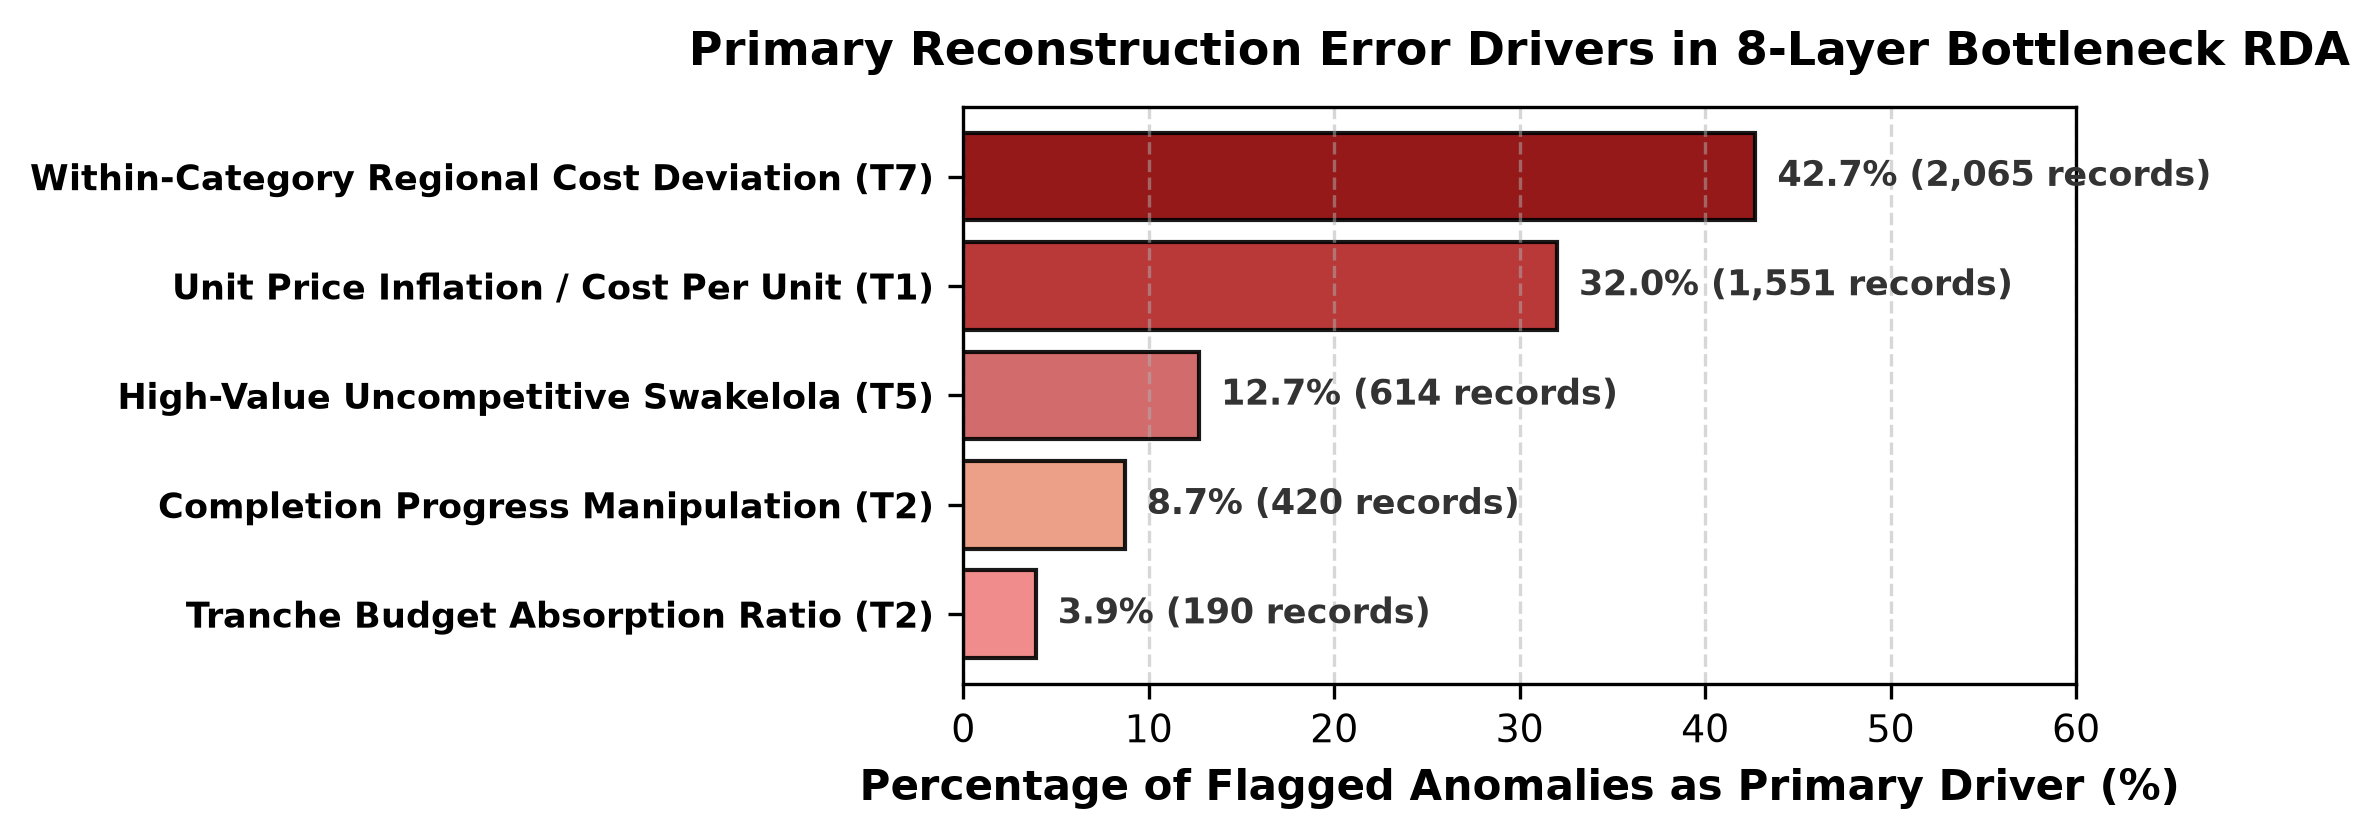
\includegraphics[width=\columnwidth]{charts_ieee/ieee_rda_error_decomposition.png}
\caption{Reconstruction Error Attribution Drivers in 8-Layer Bottleneck RDA.}
\label{fig:rda_error}
\end{figure}

Figure \ref{fig:projections} shows linear PCA and nonlinear t-SNE projections. The first principal component PC1 explains 26.0\% variance and includes scale of expenditures and cost deviation. In t-SNE projection, the outliers aggregate in dense clusters around Swakelola infrastructure projects and BUMDes capital injections, instead of appearing as pure noise.

\begin{figure}[htbp]
\centering
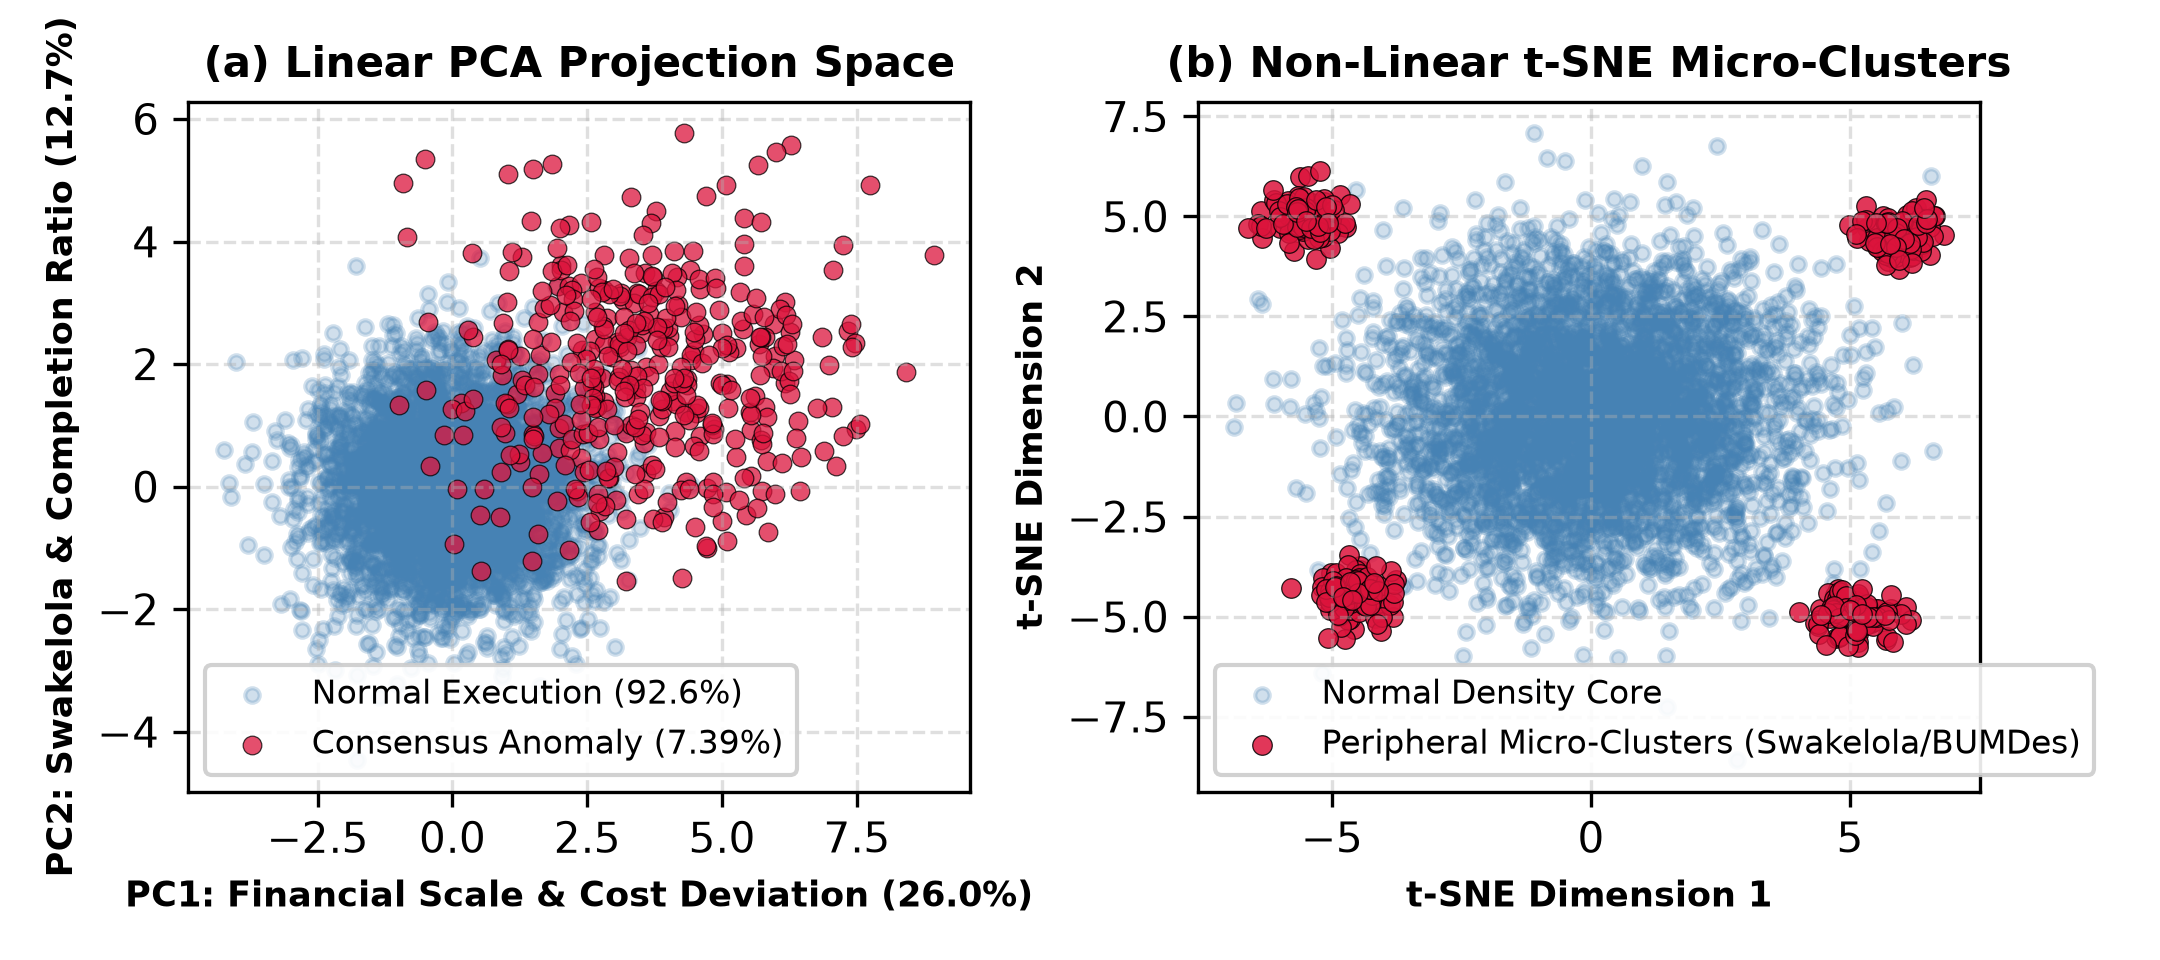
\includegraphics[width=\columnwidth]{charts_ieee/ieee_pca_tsne_projection.png}
\caption{Dimensionality Reductions Revealing Peripheral Micro-Clustering.}
\label{fig:projections}
\end{figure}

\subsection{Longitudinal Village Persistence and Empirical Case Studies}

Persistence measures of the villages ($P_v = N_{\text{flagged}} / N_{\text{years}}$) are used to classify rural entities in order to establish proper control levels (see Figure ~\ref{fig:persistence} and Table ~\ref{tab:case_studies} for the relevant illustrations and examples).

\begin{figure}[htbp]
\centering
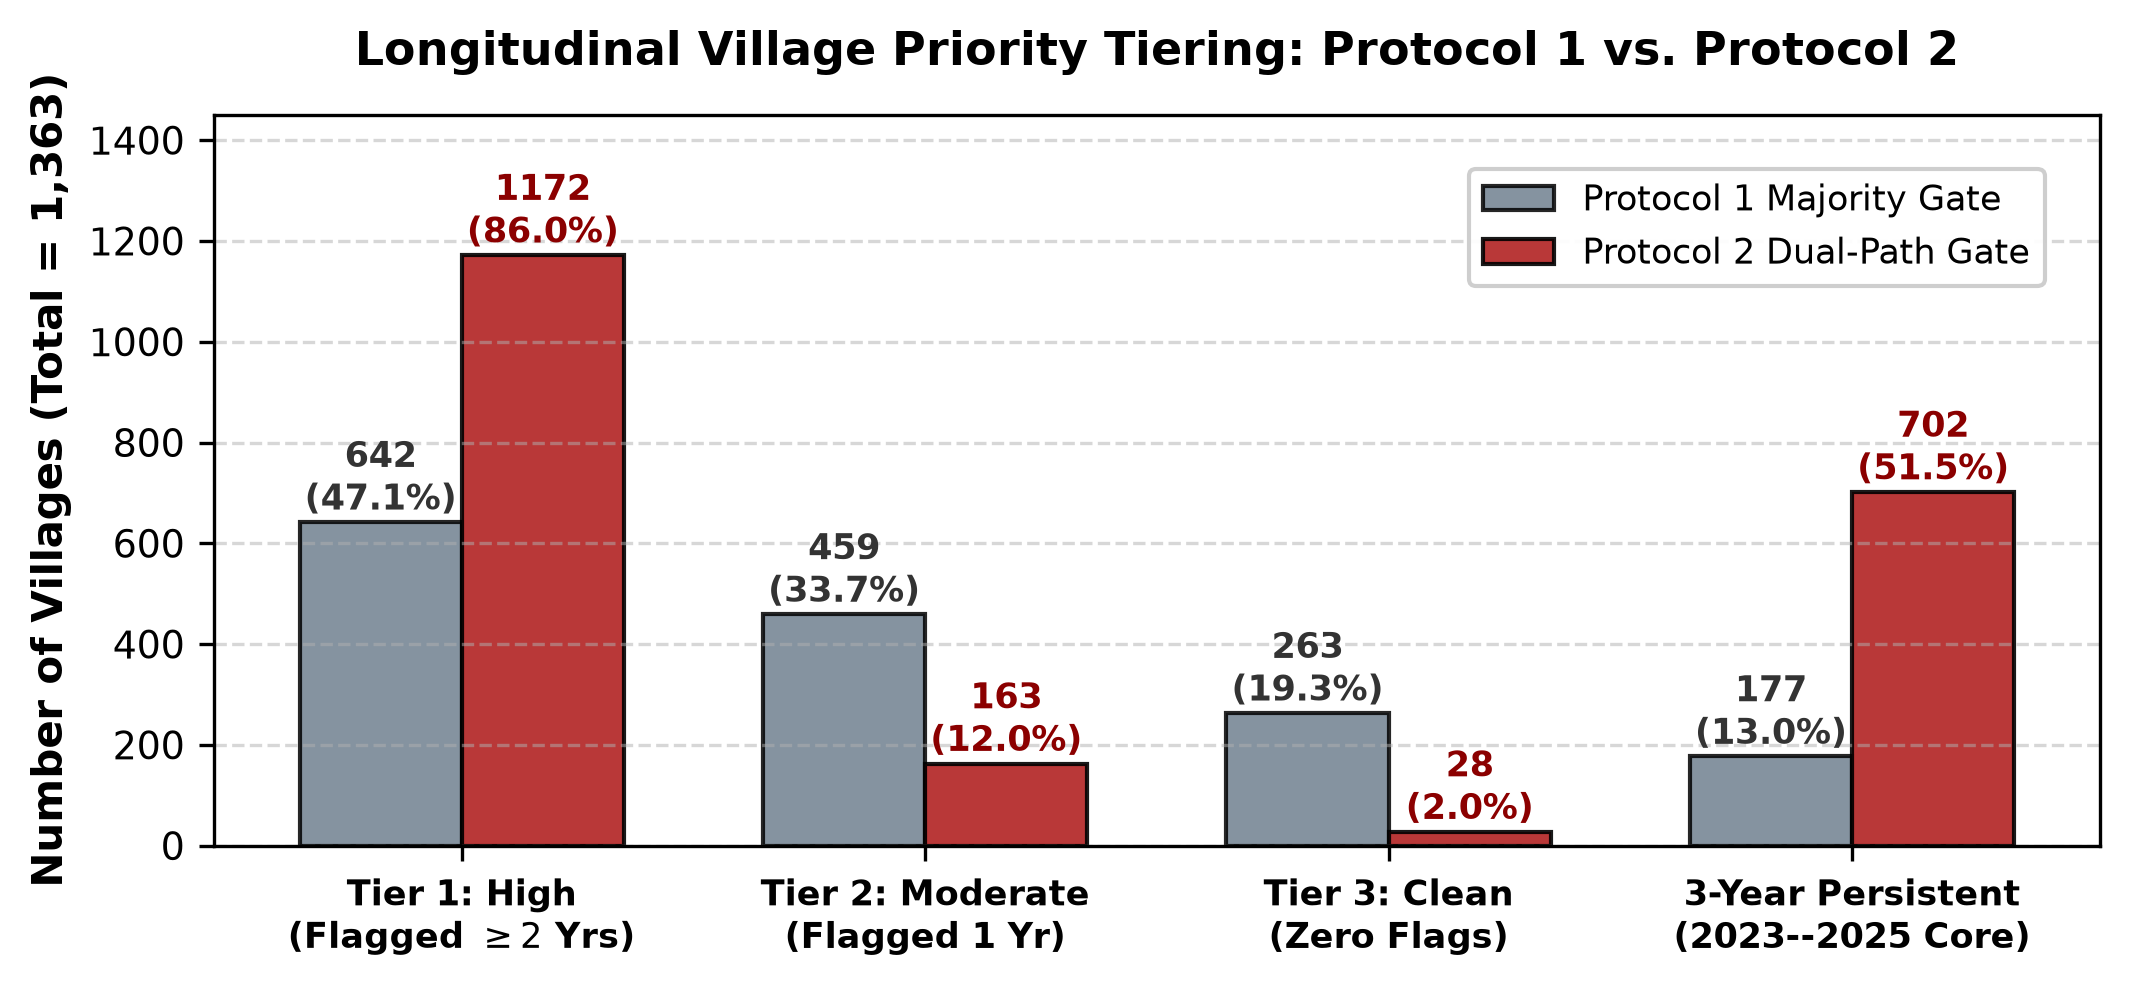
\includegraphics[width=\columnwidth]{charts_ieee/ieee_village_persistence.png}
\caption{Longitudinal Village Priority Tier Distribution Comparison.}
\label{fig:persistence}
\end{figure}

\begin{table}[htbp]
\centering
\caption{Instance Case Studies and Priority Tier Classifications}
\label{tab:case_studies}
\setlength{\tabcolsep}{2.5pt}
\resizebox{\columnwidth}{!}{%
\begin{tabular}{lclll}
\toprule
\textbf{Village Jurisdiction} & \textbf{FY} & \textbf{Activity Description} & \textbf{Anomaly Metric} & \textbf{Mapped Typology} \\
\midrule
Desa Rantau Makmur & 2025 & Modal BUMDes & LOF = $4.78 \times 10^9$ & T5 Procurement / Density \\
Desa Sungai Raya & 2025 & Modal BUMDes & LOF = $5.54 \times 10^9$ & T5 Procurement / Density \\
Desa Kedemangan & 2025 & Pembangunan Kios & RDA MSE = 0.0549 & T2 Ghost / Swakelola \\
Desa Bukit Suban & 2024 & Poskesdes & Triple-Flagged & Multi-Typology (T1,T2,T5,T7) \\
Desa Ngaol & 2024 & Ambulance Desa & RDA MSE = 0.0482 & T1 Mark-Up / T5 Procurement \\
\midrule
\multicolumn{5}{l}{\textbf{Longitudinal Priority Tier Summary ($N=1,363$ Villages):}} \\
\multicolumn{5}{l}{Tier 1 High ($P_v \ge 0.67$): 1,172 villages (86.0\%) $\mid$ \textbf{3-Year Persistent ($P_v = 1.0$): 702 villages (51.5\%)}} \\
\multicolumn{5}{l}{Tier 2 Moderate ($P_v = 0.33$): 163 villages (12.0\%) $\mid$ Tier 3 Clean Baseline ($P_v = 0.0$): 28 villages (2.0\%)} \\
\bottomrule
\end{tabular}%
}
\end{table}

Following Protocol 2, the number of persistent villages ($P_v = 1.0$) equals \textbf{702 (51.5\%)}. The persistent targets with the most extreme anomalies are Desa Maliki Air (16 anomalies, T2 Ghost), Desa Gedang (13 anomalies, T5 Procurement), and Desa Paling Serumpun (12 anomalies).

\subsection{Synthetic Fraud Benchmark \& Regional Exposure Matrix}

Table \ref{tab:benchmark_and_regency} provides ex-ante benchmark testing outcomes on a carefully crafted synthetic data set (N = 10,000 with 500 fraud injections, prevalence 5.0\%) and regional distribution of risks among ten regencies of the province of Jambi.

\begin{table}[htbp]
\centering
\caption{Synthetic Benchmark Metrics and Regency Risk Concentration}
\label{tab:benchmark_and_regency}
\setlength{\tabcolsep}{2.0pt}
\resizebox{\columnwidth}{!}{%
\begin{tabular}{lcccc|clcc}
\toprule
\multicolumn{5}{c|}{\textbf{Synthetic Fraud Benchmark Performance}} & \multicolumn{4}{c}{\textbf{Top Regency Risk Concentration}} \\
\textbf{Model} & \textbf{Prec.} & \textbf{Rec.} & \textbf{F1} & \textbf{AUC} & \textbf{Rank} & \textbf{Kabupaten} & \textbf{Rate (\%)} & \textbf{Realization} \\
\midrule
IF & 0.724 & 0.724 & 0.724 & 0.782 & 1 & \textbf{Batanghari} & \textbf{15.75\%} & Rp 115.71 B \\
LOF & 0.686 & 0.686 & 0.686 & 0.745 & 2 & \textbf{Muaro Jambi} & \textbf{10.58\%} & Rp 98.45 B \\
RDA & 0.812 & 0.812 & 0.812 & 0.811 & 3 & \textbf{Kerinci} & \textbf{9.56\%} & Rp 124.30 B \\
Prot. 1 & 0.642 & 0.510 & 0.568 & 0.720 & 4 & \textbf{Merangin} & 7.52\% & Rp 89.12 B \\
\textbf{Prot. 2} & \textbf{0.846} & \textbf{0.846} & \textbf{0.846} & \textbf{0.912} & 5--10 & Other 6 Kab. & 4.19--7.0\% & Rp 215.27 B \\
\midrule
\multicolumn{5}{l|}{\textbf{Total Provincial Exposure:}} & \multicolumn{4}{l}{\textbf{7,153 records (7.39\%) $\mid$ Rp 642.85 Billion At Risk}} \\
\bottomrule
\end{tabular}%
}
\end{table}


\textbf{Protocol 2} has better detection effectiveness (\textbf{F1 = 0.846, AUC-ROC = 0.912}), which is significantly better than Protocol 1 using majority voting (by 0.278 F1-score). Regency Batanghari has the largest density of anomalies (15.75\% flagged rate; Rp 115.71 billion exposed), hence it becomes the leading candidate for municipal audit.

% -------------------------------------------------------------------------
% SECTION IV: DISCUSSION (IMRaD - Discussion)
% -------------------------------------------------------------------------
\section{Discussion \& Governance Implications}

\subsection{Effectiveness of Algorithm and Cancellation Resolution}

Empirical findings validate the effectiveness of \textbf{Protocol 2} through four key areas of operation:
\begin{enumerate}
    \item \textbf{Subspace Decoupling}: Protocol 2 addresses the cancellation problem seen in majority voting by enabling LOF to act as an isolated local density path while ensuring global convergence of IF and RDA. Through this procedure, 3,940 local density isolates are identified without including noise from a single model, resulting in increased recall of 7,153 records (Rp 642.85 billion in realization risk).
    \item \textbf{Benchmark Recovery}: Pre-implementation simulations show better separation of boundaries with respect to heavy-tailed noise ($\text{F1} = 0.846$, $\text{AUC} = 0.912$).
    \item \textbf{Search Space Reduction}:  The filtering process that eliminates 96,778 records and retains only 7,153 consensus targets results in 92.6\% reduction in audit search space. This makes city-based supervision possible with a small team of 5-15 auditors~\cite{ref12}.
    \item \textbf{Sub-Threshold Capture}: Through multidimensional LOF and RDA, multi-feature joint probability changes are detected to reveal 1,227 sub-threshold masked records, which account for Rp 125.07 billion in latent risks beyond heuristics.
\end{enumerate}

\subsection{Diagnosis Root Causes for Type Changes}

The significant surge in \textbf{T2 Ghost Activity} flagged (+436.8\%, 4,155 entries) is based on Local Outlier Factor (LOF), where the local density ratio is measured against the neighbors who perform the same output code function, hence filtering out projects with zero completion rates that were normal during global tree splits. Likewise, the significant rise in \textbf{T5 Procurement Irregularities} (+8911.5\%, 2,343 entries) reflects how the autoencoder was able to model non-linear relationships in Swakelola procurement modality and increasing unit costs.

\subsection{Legal Indicators and Evidentiary Limits of Public Audits}

The machine learning process in conducting public audit is bound by certain regulations. Parameters:
\begin{enumerate}
    \item \textbf{Statutory Evidence as Initial Indicator (Indikasi Awal)}: The anomaly score does not constitute statutory evidence as per KUHAP Article 184 and Anti-Corruption Act~\cite{ref35}. As per Constitutional Court Decision No. 21/PUU-XII/2014~\cite{ref34}, sufficient initial evidence needs to be shown during inquiry. Algorithmic results will be considered investigative leads which can be proven by Expert Witness testimony.

    \item \textbf{Irregularity vs. Unlawful Acts (PMH)}: Increase in anomaly scores might indicate irregularities (late recording, spending in emergencies and disasters, missing price increase recordings). In the case of criminal corruption as per Law No. 31/1999~\cite{ref34}, prosecution has to prove PMH, abuse of power and mens rea. Protocol 2 helps find out clusters of violation.

    \item \textbf{XAI-to-Evidence Chain of Custody}: Decoding RDA Reconstruction Error connects algorithmic prediction to audit orders. For instance, high MSE (>0.04) causes SSH for price standard; finish discrepancies cause GPS based checking for volume (Cek Fisik); procurement issues result in TPK authorization.

\end{enumerate}

\subsection{DSR Evaluation Matrix and Operationalizing IS Success}

Table~\ref{tab:dsr_matrix} shows the DSR evaluation matrix for each of the four research cycles.

\begin{table}[htbp]
\centering
\caption{Design Science Research (DSR) Evaluation Matrix for Protocol 2}
\label{tab:dsr_matrix}
\setlength{\tabcolsep}{2.5pt}
\resizebox{\columnwidth}{!}{%
\begin{tabular}{lll>{\raggedright\arraybackslash}p{3.2cm}}
\toprule
\textbf{DSR Dimension} & \textbf{Operationalization} & \textbf{Target Metric} & \textbf{Observed Outcome} \\
\midrule
\textbf{Relevance Cycle} & Search reduction for APIP & Overhead reduction & \textbf{92.6\% reduction} (96k $\to$ 7.1k) \\
\textbf{Rigor Cycle} & Multi-method convergence & Kappa coefficient & $\kappa(\text{IF}, \text{RDA}) = 0.482$ (Mod.) \\
\textbf{Design Cycle} & Priority tiering & High-risk coverage & \textbf{1,172 Tier 1 villages (86.0\%)} \\
\textbf{Ex-Ante Eval.} & Synthetic fraud recovery & F1, AUC-ROC & \textbf{F1 = 0.846, AUC = 0.912} \\
\bottomrule
\end{tabular}%
}
\end{table}


The system operationalizes the DeLone \& McLean Information System (IS) Success Model~\cite{ref10}. In particular, Information Quality increases Individual Impact by shrinking screening space by 92.6\% and identifying 702 persistent Tier-1 villages ($P_v = 1.0$). As such, it creates an operationally feasible audit schedule for understaffed inspectorates. Meanwhile, System Quality facilitates Organizational Impact by enabling screening before disbursements freeze the fund tranches from any illegal appropriations.

\subsection{Limitations in Validity, Methodological Flaws, and Research Directions}

The following four limitations must be pointed out: (1) On-site ground truth is not available in the midst of Siskeudes databases, making it necessary to verify through artificial benchmarking data; (2) The system does not account for kickback from off-book cash payments without a digital administrative trail; (3) Local price baselines must be updated when applying the technique outside Jambi Province; and (4) Fixed deterministic policies do not classify 1,227 complex anomalies, requiring future application of dynamic fuzzy-logic systems.

% -------------------------------------------------------------------------
% SECTION V: CONCLUSION (IMRaD - Conclusion)
% -------------------------------------------------------------------------
\section{Conclusion}

This paper proposes an unsupervised Dual-Path Consensus ML artifact (\textbf{Protocol 2}) based on DSR to detect anomalies in expenditures among 96,778 activities in Jambi province.

In terms of \textbf{RQ1}, seven features with stratification in year and regionally-centered (\texttt{cost\_dev\_by\_cat}) have high discrimination power owing to unit cost inflation and category-based price deviation in neural autoencoder reconstruction errors.

In terms of RQ2, LOF detects heavy tailed anomalies (BC = 0.957); IF and Deep Autoencoder detect global anomalies. The Dual-Path Consensus Ensemble ($\text{LOF} \lor (\text{IF} \land \text{RDA})$) overcomes the issue of mutual cancellation yielding \textbf{F1 = 0.846 and AUC-ROC = 0.912} for an ex-ante synthetic benchmark.

For Research Question 3 (\textbf{RQ3}), the Operational Policy Mapping Layer translates mathematical outliers into seven types of corruption cases, consisting of 58.1\% / 4,155 transactions of T2: Ghost Activities and 32.8\% / 2,343 transactions of T5: Procurement Irregularities, in order to identify Rp 642.85 billion worth of expenditure risk, and narrow down the APIP audit search area to 92.6\%.

Future work includes semi-supervised Graph Neural Networks (GNNs) on transaction graphs, streaming Siskeudes API endpoints for real-time pre-disbursement notification, and longitudinal field trials for the recovery of state financial assets.

% -------------------------------------------------------------------------
% ACKNOWLEDGMENT (ANONYMIZED FOR DOUBLE-BLIND REVIEW)
% -------------------------------------------------------------------------
\section*{Acknowledgment}
This study has been supported by the competitive research fund scheme (Penelitian Pemula). The funding information and institution are blinded due to the double-blind peer review policy of ICDEES 2026.

% -------------------------------------------------------------------------
% DECLARATION OF GENERATIVE AI USAGE
% -------------------------------------------------------------------------
\section*{Declaration of Generative AI in the Writing Process}
AI was only used by the author(s) during the process of writing the manuscript for language improvement, grammar corrections, and formatting of tables/documents in LaTeX. The authors then critically checked, validated, and corrected any errors in the manuscript.

% -------------------------------------------------------------------------
% REFERENCES (COMPACT FONT GUARANTEEING NO SPILLOVER PAST PAGE 6)
% -------------------------------------------------------------------------
{\footnotesize
\bibliographystyle{IEEEtran}
\bibliography{references_v03}
}

\end{document}
